\chapter{Lecture}\label{part3:lec30} %%% 30
\markboth{\thechapter. Lecture}{\thechapter. Lecture}

Last\pageoriginale time we had the formula of transformation of $\log
\eta$ in the following shape:
$$
\log \eta \left( \frac{h' + i/\mathfrak{z}}{k}\right)= \log \eta
\left( \frac{h + i \mathfrak{z}}{k}\right) + \frac{1}{2} \log z +
\frac{\pi i}{12k} (h' -h) + \pi i s(h, k),
$$
where $s(h, k)$ is the Dedekind sum, which, by direct computation of
residues, was seen to be
$$
\sum^{k-1}_{\mu=0} \left(\frac{\mu}{k} - \frac{1}{2} \right) \left(
\frac{h \mu}{k} - \left[ \frac{h \mu}{k}\right]- \frac{1}{2}\right).
$$

We use the abbreviation: for real $x$,
$$
((x)) =
\begin{cases}
  x- & [x]  - \frac{1}{2}, \text{if $x$ is not an integer,}\\
    & 0  ~~\qquad , \text{if $x$ is an integer.}
\end{cases}
$$

Then 
$$
s(h, k) = \sum^k_{\mu=1} \left( \left(\frac{\mu}{k} \right) \right)
\left( \left( \frac{h \mu}{k}\right) \right).
$$

Now $((x))$ is an odd function; for $x$ integer, trivially $((-x))=-
((x))$, and for $x$ not an integer,
\begin{align*}
  ((-x)) & = - x - [-x]- \frac{1}{2}\\
  & =- x + [x] +1- \frac{1}{2}, ~\text{since}~ [-x]=- [x] -1,\\
  & = - ((x)).\\
********* & **************
\end{align*}

$((x))$\pageoriginale is the familiar function whose graph is as
indicated. 

\begin{figure}[H]
  \centering{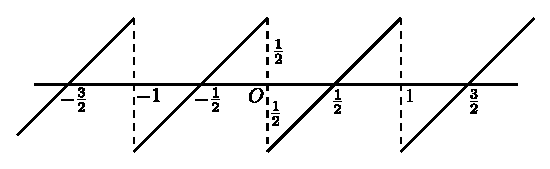
\includegraphics{vol2-figures/fig2.37.eps}}
\end{figure}

We now prove that
$$
\sum^k_{\mu=1} \left( \left( \frac{\mu}{k}\right) \right)=0
$$

Because of periodicity we can write
\begin{align*}
  \sum^k_{\mu=1} \left( \left( \frac{\mu}{k}\right) \right) & =
  \sum_{\mu \mod k} \left( \left( \frac{\mu}{k}\right) \right)\\
  & = \sum_{\mu \mod k} \left(\left(\frac{\mu}{k} \right)\right)\\
  & = - \sum_{\mu \mod k} \left( \left(\frac{\mu}{k} \right) \right)\\
  \therefore \quad \sum^k_{\mu =1} \left( \left( \frac{\mu}{k} \right)
  \right) & =0
\end{align*}

We can also write $s(h, k)$ in the form
\begin{align*}
  s(h, k) & = \sum^k_{\mu=1} \left( \frac{\mu}{k} - \frac{1}{2}\right)
  \left( \left( \frac{h \mu}{k}\right) \right) \\
  & = \sum^k_{mu=1} \frac{\mu}{k} \left( \left( \frac{h \mu}{k}
  \right) \right) - \frac{1}{2} \sum^k_{\mu=1} \left( \left(\frac{h
    \mu}{k}  \right) \right),
\end{align*}
and\pageoriginale since $h \mu$ also runs through a full system of
residues $\mod k$ when $\mu$ does so, as $(h, k)=1$, the second sum is
zero, and we can therefore write
$$
s(h, k) = \sum^k_{\mu=1} \frac{\mu}{k} \left( \left( \frac{h
  \mu}{k}\right) \right) 
$$

Let us now rewrite this in a form in which the modular substitution
comes into play
$$
\tau' = \frac{h' + i /\mathfrak{z}}{k}, \quad \tau= \frac{h + i
  \mathfrak{z}}{k}; 
$$
so $k \tau - h = i \mathfrak{z}$, and 
\begin{align*}
  \tau' & = \frac{h' - 1/(k \tau -h)}{k} = \frac{h' k \tau - h h'-1}{k
    (k \tau -h)} \\
  & = \frac{h' \tau - (h h'+1)/k}{k \tau-h} 
\end{align*}
($\frac{h h'+1}{k}$ is necessarily integral for $h h' \equiv -1 \mod
k$). So the modular substitution is 
$$
\begin{pmatrix}
  h' & \frac{-hh'+1}{k}\\
  k & -h
\end{pmatrix}= 
\begin{pmatrix}
  a & b\\
  c & d
\end{pmatrix}, c > 0.
$$

The transformation formula for $\log \eta$ now reads
$$
\log \eta \left( \frac{a \tau+ b}{c \tau+d}\right) = \log \eta (\tau)
+ \frac{1}{2} \log \frac{c \tau +d}{i} + \frac{\pi i}{12c} (a+d) - \pi
i s (d, c),
$$
since $s(-d, c)=- -s(d, c)$.

Let\pageoriginale us take in particular
$$
\begin{pmatrix}
  a & b\\
  c & d
\end{pmatrix}= 
\begin{pmatrix}
  0 & -1\\
  1 & 0
\end{pmatrix};
$$
then we obtain 
$$
\log \eta \left( \frac{1}{\tau}\right)= \log \eta (\tau) + \frac{1}{2}
\log \frac{\tau}{i},
$$
the special case discussed by Siegel.

Let us now make two substitutions in succession: 
$$
\tau'' = \frac{a \tau'+b}{c \tau' +d}, \quad \tau' =- \frac{1}{\tau}.
$$
Then
$$
\tau'' = \frac{-a/\tau +b}{-c/\tau+d} = \frac{b \tau -a}{d \tau -c}
$$

We suppose $c> 0$, $d> 0$; $(c, d)=1$. Then
\begin{align*}
  \log \eta(\tau'')& = \log \eta (\tau') + \frac{1}{2} \log \frac{c
    \tau'+d}{i} + \frac{\pi i}{12c} (a+d)- \pi i s(d,c);\\
  \log \eta (\tau'') & = \log \eta (\tau) + \frac{1}{2} \log \frac{d
    \tau -c}{i} + \frac{\pi i}{12d} (b-c) - \pi i s(-c, d).
\end{align*}

Sub tracting, and observing that 
$$
\log \eta (\tau') - \log \eta n (\tau) = \frac{1}{2} \log \frac{\tau}{i},
$$
we\pageoriginale have
\begin{multline*}
  0 = \frac{1}{2} \log \frac{\tau}{i} + \frac{1}{2} \log \frac{c \tau'
    +d}{i} - \frac{1}{2} \log \frac{d \tau -c}{i}\\ 
  + \frac{\pi i}{12}
  \left( \frac{a+d}{c}- \frac{b-c}{d}\right) - \pi i (s (d,c)- s(c, d))
\end{multline*}

The sum of the logarithms on the right side is determinate only up to
a multiple of $2 \pi i$:
\begin{align*}
  \log \frac{\tau}{1} + \log \frac{c \tau' +d}{i} - \log \frac{d
    \tau-c}{i} & = \log \frac{\tau}{i} \frac{(- c/\tau + d)/i}{(d \tau
    -c)/i} + 2 \pi i k\\
  & = \log \left( \frac{1}{i}\right) +2 \pi i k\\
  & = - \frac{\pi i}{2} + 2 \pi i k
\end{align*}

Now each logarithm above has an imaginary part which is strictly less
than $\frac{\pi}{2}$ in absolute value; so
$$
\left| Im \left\{ \log \frac{\tau}{i} + \log \frac{c
  \tau'+d}{i} - \log \frac{d \tau-c}{i}\right\}\right| < \frac{3 \pi}{2}
$$

So the only admissible value of $k$ is zero.

Hence\pageoriginale we have
$$
0= - \frac{\pi i}{4} + \frac{\pi i}{12} \left(\frac{a+d}{c} -
\frac{b-c}{d} - \pi i (s(d,c) + s(c, d)) \right),
$$
or since $ad-bc=1$,
$$
s(d, c)+ s(c, d)= - \frac{1}{4} + \frac{1}{12} \left( \frac{d}{c} +
\frac{c}{d} +\frac{1}{cd}\right).  
$$

This is the reciprocity law for Dedekind sums. It is a purely
arithmetical formula for which I have given several proofs; here I
reproduce the proof that I gave originally, by lattice-point
enumeration. 

We have to prove that
$$
\displaylines{\sum^{k-1}_{\mu=1} \frac{\mu}{k} \left\{ \frac{h \mu}{k}
  - \left[\frac{h \mu}{k} \right]- \frac{1}{2}\right\}+
  \sum^{h-1}_{\mu=1} \frac{\nu}{h} \left\{\frac{k \nu}{h}-
  \left[\frac{h \nu}{k} \right] - \frac{1}{2}\right\}\cr
  = - \frac{1}{4} + \frac{1}{12} \left(\frac{h}{k} + \frac{k}{h} +
  \frac{1}{hk} \right),\cr
  \text{or} \hfill \cr
  \frac{h}{k^2} \sum^{k-1}_{\mu-1} \mu^2 - \frac{1}{2k}
  \sum^{k-1}_{\mu-1} \mu + \frac{k}{h^2} \sum^{h-1}_{\nu-1} \nu^2 -
  \frac{1}{2h} \sum^{h-1}_{\nu=1} \nu - \frac{1}{k} \sum^{k-1}_{\mu=1}
  \mu \left[ \frac{h \mu}{k}\right] - \frac{1}{h} \sum^{h-1}_{\nu=1}
  \nu \left[ \frac{k \nu}{h}\right]\cr
  =- \frac{1}{4} + \frac{1}{12} \left( \frac{h}{k} + \frac{h}{h} +
  \frac{1}{hk}\right);}
$$
\noindent
or\pageoriginale 
$$
\displaylines{
  \frac{h^2 (k-1)(2k-1)}{6} - \frac{h}{2} \frac{k(k-1)}{2} + \frac{k^2
    (h-1)(2h-1)}{6}- \frac{k}{2} \frac{h(h-1)}{2}\hfill \cr 
  \hfill - h
  \sum^{k-1}_{\mu=1} \mu \left[ \frac{h \mu}{k}\right]- k
  \sum^{h-1}_{\nu=1} \nu \left[ \frac{k \nu}{h}\right]\cr
  = \frac{- 3 hk + h^2 + k^2 +1}{12}\cr
  \text{i.e.,} \hfill 12 h \sum^{k-1}_{\mu=1} \mu \left[\frac{h
      \mu}{k} \right] + 12k \sum^{h-1}_{\nu=1} \nu \left[\frac{k
      \nu}{h} \right]\hfill \cr
  = h(k-1)(2h(2k-1)-3k)+ k (h-1)(2k (2h-1)-3h)+ 3hk-h^2 -k^2 -1\hfill \cr
  = 8 h^2 k^2 - 9 h^2 k - 9 hk^2 + h^2 + k^2 + 9  hk-1\hfill \cr
  = (h-1)(k-1)(8hk -h -k -1)\hfill  }
$$

So the whole thing is equivalent to proving that
$$
12h \sum^{k-1}_{\mu=1} \mu \left[\frac{h \mu}{k} \right] + 12k
\sum^{h-1}_{\nu=1} \nu \left[\frac{k \nu}{h} \right] = (h-1)(k-1)(8hk-h-k-1).
$$

This reduces to something that looks familiar; indeed the square
brackets appear in lattice-point enumeration. Here $(h, k)=1$, but in
a paper with Whiteman I have also discussed the case where $h, k$ are
not coprime.

Enumerating\pageoriginale by rows and columns parallel  to the $\mu-$
and $\nu-$ axes, the number of lattice-points in the integer a the
rectangle 
\begin{figure}[H]
  \centering{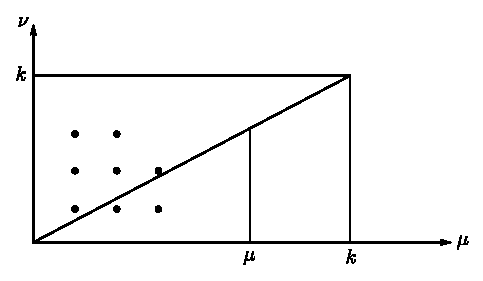
\includegraphics{vol2-figures/fig2.38.eps}}
\end{figure}

\noindent with sides of length $k, h$ along the axes of $\mu$ and
$\nu$ respectively is seen to be $(h-1)(k-1)$. This can be enumerated
in another way also. The number of lattice points in the interior,
with abscissa $\mu$ and lying below the diagonal through the origin is
the full integer in $\frac{h \mu}{k}$. So we have $\sum\limits^{k-1}_{\mu=1}
\left[ \frac{h \mu}{k}\right]$ lattice points below the
diagonal. Similarly there are $\sum\limits^{h-1}_{\nu =1} \left[\frac{k
    \nu}{h} \right]$ points above the diagonal. Since $(h, k)=1$ there
are no points on the diagonal. Hence
$$
(h-1)(k-1) = \sum^{k-1}_{\mu=1} \left[ \frac{h \mu}{k}\right] +
\sum^{h-1}_{\nu=1} \left[ \frac{k \nu}{h}\right]
$$

In out case we have quadratic summands; but something which goes so
well here in the plane should go well in space also.

